\documentclass{beamer}
\usepackage{amsmath}
\usepackage{amssymb}
\usepackage{tikz}
\usepackage{booktabs}

% Theme
\usetheme{Madrid}
\usecolortheme{default}

% Title page info
\title{Collaborative Filtering with Matrix Factorization}
\subtitle{Book Recommendation System}
\author{Hardcover Book Friend Finder}
\date{\today}

\begin{document}

% Title slide
\begin{frame}
\titlepage
\end{frame}

% Table of contents
\begin{frame}{Outline}
\tableofcontents
\end{frame}

% ============================================================================
\section{Introduction}
% ============================================================================

\begin{frame}{Overview}
\begin{block}{Goal}
Build a personalized book recommendation system using collaborative filtering
\end{block}

\vspace{0.5cm}

\begin{columns}[T]
\column{0.5\textwidth}
\textbf{Dataset:}
\begin{itemize}
    \item 1,000 users collected
    \item 45,203 books
    \item 95.75\% sparse
\end{itemize}

\column{0.5\textwidth}
\textbf{Results:}
\begin{itemize}
    \item 8.83\% precision
    \item 308\% better than pure collaborative filtering
    \item ~5 second training time
\end{itemize}
\end{columns}
\end{frame}

% ============================================================================
\section{Data Preparation}
% ============================================================================

\begin{frame}{Dataset Statistics}
\begin{columns}[T]
\column{0.5\textwidth}
\textbf{Raw Dataset:}
\begin{itemize}
    \item 1,000 users collected
    \item 45,203 books
    \item Avg: 84.4 books/user
    \item Median: 1.0 books/user
\end{itemize}

\column{0.5\textwidth}
\textbf{After Filtering:}
\begin{itemize}
    \item 246 users (24.6\%)
    \item 2,547 books (5.6\%)
    \item Avg: 113.8 books/user
    \item 26,598 interactions
\end{itemize}
\end{columns}

\vspace{0.5cm}

\begin{block}{Filtering Criteria}
\begin{itemize}
    \item \textbf{Users}: $\geq 20$ book interactions
    \item \textbf{Books}: $\geq 5$ users
    \item \textbf{Why?} Better signal-to-noise ratio
\end{itemize}
\end{block}

\vspace{0.3cm}

\textbf{Matrix Sparsity:} 95.75\% (626,562 possible, 26,598 actual)
\end{frame}

\begin{frame}{Feedback Distribution}
\textbf{26,598 total interactions broken down by type:}

\vspace{0.5cm}

\begin{table}
\centering
\begin{tabular}{lrr}
\toprule
\textbf{Type} & \textbf{Count} & \textbf{Percentage} \\
\midrule
Read & 16,340 & 61.4\% \\
Want to Read & 12,102 & 45.5\% \\
Currently Reading & 289 & 1.1\% \\
DNF & - & - \\
\bottomrule
\end{tabular}
\end{table}

\vspace{0.3cm}

\begin{block}{Implicit Feedback Impact}
Adding "want to read" + "currently reading" increased training data by \alert{75\%}!
\end{block}
\end{frame}

% ============================================================================
\section{Matrix Factorization}
% ============================================================================

\begin{frame}{The Core Idea}
\begin{block}{Matrix Decomposition}
Factor the sparse user-book matrix $Y$ into two smaller matrices:
\end{block}

\begin{equation*}
Y_{m \times n} \approx \sigma(X_{m \times k} \cdot W_{n \times k}^T + b)
\end{equation*}

\vspace{0.5cm}

\begin{columns}[T]
\column{0.5\textwidth}
\textbf{Dimensions:}
\begin{itemize}
    \item $m = 2,547$ books
    \item $n = 246$ users
    \item $k = 20$ features
\end{itemize}

\column{0.5\textwidth}
\textbf{Matrices:}
\begin{itemize}
    \item $X$: Book features
    \item $W$: User features
    \item $b$: User bias
    \item $\sigma$: Sigmoid activation
\end{itemize}
\end{columns}
\end{frame}

\begin{frame}{Matrix Multiplication Diagram}
\begin{center}
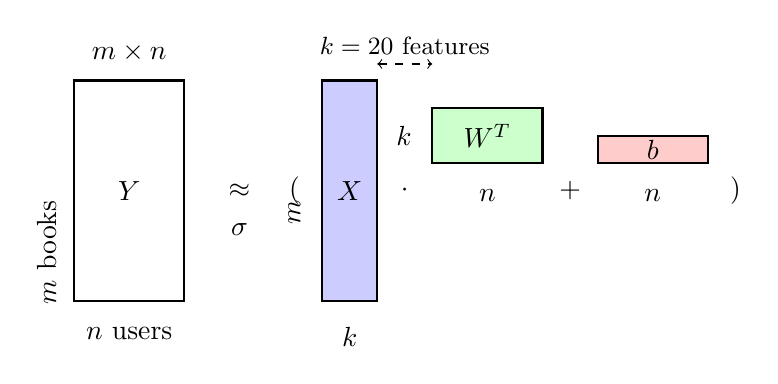
\begin{tikzpicture}[scale=0.7]
    % Y matrix
    \draw[thick] (0,0) rectangle (2,4);
    \node at (1,2) {$Y$};
    \node[below] at (1,-0.3) {$n$ users};
    \node[left,rotate=90] at (-0.5,2) {$m$ books};
    \node at (1,4.5) {$m \times n$};

    % Approximately equal
    \node at (3,2) {$\approx$};
    \node at (3,1.3) {$\sigma$};

    % Opening parenthesis
    \node at (4,2) {$($};

    % X matrix
    \draw[thick,fill=blue!20] (4.5,0) rectangle (5.5,4);
    \node at (5,2) {$X$};
    \node[below] at (5,-0.3) {$k$};
    \node[left,rotate=90] at (4,2) {$m$};

    % Multiplication dot
    \node at (6,2) {$\cdot$};

    % W^T matrix
    \draw[thick,fill=green!20] (6.5,2.5) rectangle (8.5,3.5);
    \node at (7.5,3) {$W^T$};
    \node[below] at (7.5,2.2) {$n$};
    \node[left] at (6.3,3) {$k$};

    % Plus
    \node at (9,2) {$+$};

    % b vector
    \draw[thick,fill=red!20] (9.5,2.5) rectangle (11.5,3);
    \node at (10.5,2.75) {$b$};
    \node[below] at (10.5,2.2) {$n$};

    % Closing parenthesis
    \node at (12,2) {$)$};

    % Feature dimension annotations
    \draw[<->,dashed] (5.5,4.3) -- (6.5,4.3);
    \node[above] at (6,4.3) {\small $k=20$ features};
\end{tikzpicture}
\end{center}
\end{frame}

\begin{frame}{Latent Features}
\textbf{What are the $k=20$ latent features?}

\vspace{0.5cm}

\begin{block}{Book Features ($X$)}
Each book gets a 20-dimensional vector representing:
\begin{itemize}
    \item Genre (fantasy, sci-fi, literary fiction)
    \item Reading level
    \item Themes and topics
    \item Popularity
\end{itemize}
\end{block}

\begin{block}{User Features ($W$)}
Each user gets a 20-dimensional vector representing:
\begin{itemize}
    \item Affinity for each latent dimension
    \item Reading preferences
    \item Taste profile
\end{itemize}
\end{block}

\textbf{Key:} These features are \alert{learned automatically} through gradient descent!
\end{frame}

% ============================================================================
\section{Handling Sparsity}
% ============================================================================

\begin{frame}{The Masking Approach}
\textbf{Problem:} 95.75\% of the matrix is unread books!

\vspace{0.5cm}

\begin{block}{Solution: Mask Matrix $R$}
\begin{equation*}
R_{ij} = \begin{cases}
1 & \text{if user } j \text{ interacted with book } i \\
0 & \text{otherwise}
\end{cases}
\end{equation*}
\end{block}

\vspace{0.3cm}

\begin{block}{Rating Scale with Implicit Feedback}
\begin{equation*}
Y_{ij} = \begin{cases}
1.0 & \text{read with rating } \geq 3 \\
0.7 & \text{currently reading} \\
0.3 & \text{want to read} \\
0.0 & \text{disliked or DNF} \\
\alert{0.5} & \text{unread (ignored!)}
\end{cases}
\end{equation*}
\end{block}
\end{frame}

\begin{frame}{Masked Loss Function}
\textbf{Key Innovation:} Only train on known interactions!

\vspace{0.5cm}

\begin{block}{Cost Function}
\begin{equation*}
J = \sum_{i,j} \alert{R_{ij}} \left(\sigma(x_i^T w_j + b_j) - Y_{ij}\right)^2 + \frac{\lambda}{2}\left(\|X\|_F^2 + \|W\|_F^2\right)
\end{equation*}
\end{block}

\vspace{0.3cm}

\begin{itemize}
    \item $R_{ij}$ masks out unread books (where $Y_{ij} = 0.5$)
    \item Without masking, 95.75\% unread would dominate the loss
    \item Model would just learn the global average
\end{itemize}

\vspace{0.3cm}

\textbf{Result:} Model learns from actual preferences, not missing data!
\end{frame}

% ============================================================================
\section{Training}
% ============================================================================

\begin{frame}{Optimization}
\textbf{Algorithm:} Gradient descent with Adam optimizer

\vspace{0.5cm}

\begin{block}{Configuration}
\begin{itemize}
    \item Learning rate: $\alpha = 0.1$
    \item Regularization: $\lambda = 1.0$
    \item Iterations: 300
    \item Features: $k = 20$
\end{itemize}
\end{block}

\vspace{0.3cm}

\begin{block}{Training Time (on 246 users)}
\begin{itemize}
    \item Data loading: 1.40s
    \item Matrix building: 0.02s
    \item Model training: 3.26s
    \item User clustering: 0.04s
    \item \textbf{Total: 4.72s}
\end{itemize}
\end{block}
\end{frame}

\begin{frame}{Scalability}
\textbf{How does it scale?}

\vspace{0.5cm}

\begin{table}
\centering
\small
\begin{tabular}{rrrr}
\toprule
\textbf{Users} & \textbf{Active} & \textbf{Interactions} & \textbf{Time} \\
\midrule
1,000 & ~246 & ~26,598 & 4.4s \\
5,000 & ~1,230 & ~132,990 & 17.0s \\
10,000 & ~2,460 & ~265,980 & 32.7s \\
100,000 & ~24,600 & ~2,659,800 & \alert{5.2 min} \\
\bottomrule
\end{tabular}
\end{table}

\vspace{0.5cm}

\textbf{Complexity:} $O(\text{iterations} \times k \times m \times n)$

\textbf{Rate:} ~12.6ms per user (linear scaling)
\end{frame}

% ============================================================================
\section{Results}
% ============================================================================

\begin{frame}{Hybrid Model}
\textbf{Pure collaborative filtering only achieved 2.45\%!}

\vspace{0.5cm}

\begin{block}{Solution: Hybrid Approach}
\begin{equation*}
\text{score}_{ij} = 0.5 \cdot \text{popularity}_i + 0.5 \cdot \sigma(x_i^T w_j + b_j)
\end{equation*}
\end{block}

\vspace{0.3cm}

\textbf{Why this works:}
\begin{itemize}
    \item \textbf{Popularity (50\%)}: Ensures quality recommendations
    \item \textbf{Collaborative (50\%)}: Adds personalization
    \item \textbf{Implicit feedback}: +75\% more training data
\end{itemize}
\end{frame}

\begin{frame}{Performance Comparison}
\begin{table}
\centering
\begin{tabular}{lc}
\toprule
\textbf{Method} & \textbf{Precision@10} \\
\midrule
Pure collaborative filtering & 2.16\% \\
Improved collaborative (filtered) & 2.45\% \\
Popularity baseline & 7.56\% \\
\alert{\textbf{Hybrid (50/50)}} & \alert{\textbf{8.83\%}} \\
\bottomrule
\end{tabular}
\end{table}

\vspace{0.5cm}

\begin{block}{Improvement}
\begin{itemize}
    \item \alert{+308\%} vs pure collaborative filtering
    \item \alert{+17\%} vs popularity baseline
\end{itemize}
\end{block}
\end{frame}

% ============================================================================
\section{Comparison}
% ============================================================================

\begin{frame}{Netflix vs. Hardcover}
\begin{table}
\centering
\tiny
\begin{tabular}{p{2.5cm}p{4cm}p{4cm}}
\toprule
\textbf{Aspect} & \textbf{Netflix} & \textbf{Hardcover} \\
\midrule
Rating scale & $\{-1, 1, 0\}$ & $\{0, 0.3, 0.7, 1, 0.5\}$ \\
Unranked & 0 = unranked, predicted & 0.5 = \alert{masked out} \\
Activation & Linear ($\in \{-1,1\}$) & Sigmoid ($\in [0,1]$) \\
Loss & All entries & \alert{Only known} (R=1) \\
Sparsity & ~95-98\% & 95.75\% \\
\bottomrule
\end{tabular}
\end{table}

\vspace{0.5cm}

\textbf{Key difference:} We mask unread books, Netflix predicts them

\textbf{Why?} Our data is too sparse to predict missing values reliably
\end{frame}

% ============================================================================
\section{Friend Matching}
% ============================================================================

\begin{frame}{User Clustering}
\textbf{Goal:} Find users with similar reading preferences

\vspace{0.5cm}

\begin{block}{Method: K-means Clustering}
\begin{itemize}
    \item Cluster on L2-normalized user embeddings $W$
    \item Tested $K \in [3, 15]$ using silhouette score
    \item \alert{Optimal: $K=13$ clusters} (score: 0.084)
\end{itemize}
\end{block}

\vspace{0.3cm}

\begin{columns}[T]
\column{0.5\textwidth}
\textbf{Note:}
\begin{itemize}
    \item $k=20$ latent \textbf{features}
    \item $K=13$ \textbf{clusters}
\end{itemize}

\column{0.5\textwidth}
\textbf{Examples:}
\begin{itemize}
    \item Classic YA \& Fantasy
    \item Sci-Fi Enthusiasts
    \item Literary Fiction
\end{itemize}
\end{columns}

\vspace{0.3cm}

\textbf{Friend matching:} Cosine similarity within clusters
\begin{equation*}
\text{sim}(u_i, u_j) = \frac{w_i \cdot w_j}{\|w_i\| \|w_j\|}
\end{equation*}
\end{frame}

\begin{frame}{Cluster Size Distribution}
\textbf{13 clusters with varying sizes:}

\vspace{0.3cm}

\begin{table}
\centering
\small
\begin{tabular}{clr}
\toprule
\textbf{ID} & \textbf{Size} & \textbf{\%} \\
\midrule
7 & 52 users & 21.1\% \\
2 & 35 users & 14.2\% \\
10 & 21 users & 8.5\% \\
5 & 20 users & 8.1\% \\
1,3 & 19 users each & 7.7\% \\
13 & 17 users & 6.9\% \\
6 & 15 users & 6.1\% \\
4,8 & 12 users each & 4.9\% \\
11 & 11 users & 4.5\% \\
9 & 9 users & 3.7\% \\
12 & 4 users & 1.6\% \\
\bottomrule
\end{tabular}
\end{table}

\textbf{Largest cluster:} 21.1\% of users | \textbf{Smallest:} 1.6\%
\end{frame}

\begin{frame}{Most Popular Books}
\textbf{Top 10 books in the dataset:}

\vspace{0.3cm}

\begin{table}
\centering
\small
\begin{tabular}{rlr}
\toprule
\# & \textbf{Title} & \textbf{Users} \\
\midrule
1 & 1984 & 106 (43.1\%) \\
2 & Harry Potter and the Sorcerer's Stone & 88 (35.8\%) \\
3 & Project Hail Mary & 80 (32.5\%) \\
4 & The Hobbit & 80 (32.5\%) \\
5 & Animal Farm & 76 (30.9\%) \\
6 & The Hunger Games & 76 (30.9\%) \\
7 & To Kill A Mockingbird & 74 (30.1\%) \\
8 & Dune & 67 (27.2\%) \\
9 & The Hitchhiker's Guide to the Galaxy & 64 (26.0\%) \\
10 & Mistborn: The Final Empire & 63 (25.6\%) \\
\bottomrule
\end{tabular}
\end{table}
\end{frame}

% ============================================================================
\section{Conclusion}
% ============================================================================

\begin{frame}{Key Innovations}
\begin{enumerate}
    \item \textbf{Masking} unread books to avoid learning from noise
    \vspace{0.3cm}
    \item \textbf{Implicit feedback} to increase training signals by 75\%
    \vspace{0.3cm}
    \item \textbf{Hybrid ensemble} balancing popularity and personalization
    \vspace{0.3cm}
    \item \textbf{Low-dimensional embeddings} ($k=20$) capturing preferences
    \vspace{0.3cm}
    \item \textbf{Clustering} for friend matching (13 reading groups)
\end{enumerate}
\end{frame}

\begin{frame}{Summary}
\begin{block}{Achievement}
8.83\% precision@10 for 246 active readers
\end{block}

\vspace{0.5cm}

\begin{columns}[T]
\column{0.5\textwidth}
\textbf{Pros:}
\begin{itemize}
    \item Fast training (~5s)
    \item Scales linearly
    \item Personalized
    \item Friend matching
\end{itemize}

\column{0.5\textwidth}
\textbf{Future Work:}
\begin{itemize}
    \item Content features
    \item More implicit feedback
    \item Neural networks
    \item More users
\end{itemize}
\end{columns}

\vspace{0.5cm}

\begin{center}
\Large
\textbf{Questions?}
\end{center}
\end{frame}

\end{document}
